\documentclass[10pt, conference]{IEEEtran}
\usepackage{xeCJK}
\usepackage{amsmath}
\usepackage{listings}
\usepackage{amssymb}
\usepackage{float}
\usepackage{graphicx}

% 用来断词,当出现花括号中的单词时,若遇到换行需要断词的话就只能从-处断。
\hyphenation{op-tical net-works semi-conduc-tor}

\begin{document}
    \title{Report: Show/prove how "always" and "until" can be derived from "Weak Until"}
    \author{\IEEEauthorblockN{林奇峰, Qifeng Lin}\IEEEauthorblockA{Student ID:17214656}}
    \date{\today}
    \maketitle
    
    The assignment is to show how "always" and "until" can be derived from "Weak Until".
    \begin{align*}
      \Box\varphi &\equiv \varphi\textbf{W}\text{false} \\
      \varphi\textbf{U}\psi & \equiv(\varphi\textbf{W}\psi)\wedge\diamond\psi
    \end{align*}
    Here, we replace $\varphi$ and $\psi$ with "a" and "b".

    According to the definition of "always" and "until", the pictures below show how they perform.
    \begin{figure}[H]
      \centering
      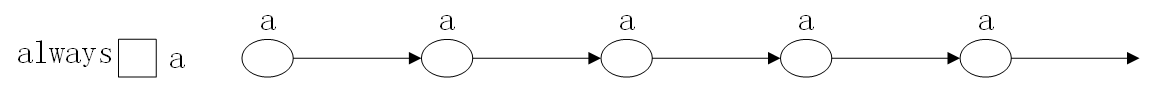
\includegraphics[width=3.0in]{3.png}
      \caption{"always"}
    \end{figure}
    \begin{figure}[H]
      \centering
      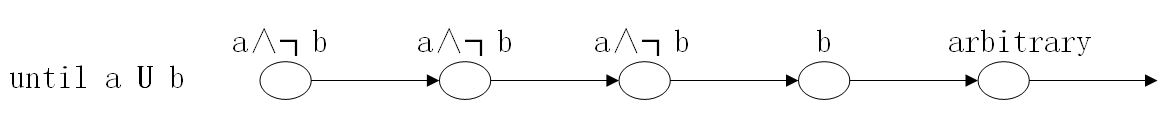
\includegraphics[width=3.0in]{1.png}
      \caption{"until"}
    \end{figure}

    We can see that "always" means that a property is always true and "until", "a {\textbf U} b", means that a is always true until b is true.

    And "weak until" can be showed as following picture
    \begin{figure}[H]
      \centering
      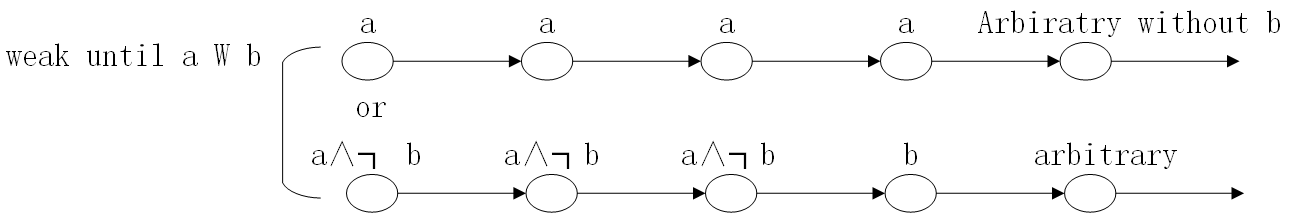
\includegraphics[width=3.0in]{4.png}
      \caption{"weak until"}
    \end{figure}
    
    We can see that "weak until", "a \textbf{W} b" can be divided into two cases: one is with b and the other one is without b.
    Therefore, for "a \textbf{W} false", we can obtain the following picture.
    \begin{figure}[H]
      \centering
      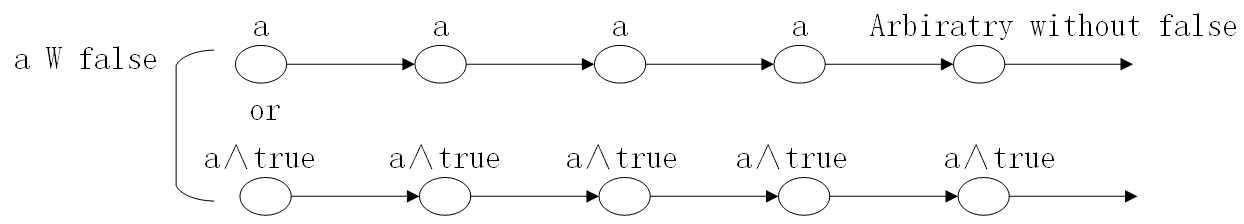
\includegraphics[width=3.0in]{5.png}
      \caption{"a \textbf{W} false"}
    \end{figure}
    
    We need to explain how to acquire the picture below. Firstly, for the first case, we can see that "a" is always true because "false" does't happen. And for the second case, since the negation of "false" is "true" and "false" means that it never occurs, it can be reasoned that "a $\wedge$ true" is always true. But "a $\wedge$ true" is equivalent to "a". Therefore, "$\Box$a" is equivalent to "a \textbf{W} false". That is, $\Box\varphi\equiv \varphi\textbf{W}\text{false}$.
    
   As for "(a \textbf{W} b)$\wedge\diamond$b", since "$\wedge\diamond$b" guarantees the occurrence of b, the first case of "(a \textbf{W} b)" is excluded and the second case remains. The second case is the form of "a \textbf{W} b". The statement before can be showed as picture below.
   \begin{figure}[H]
      \centering
      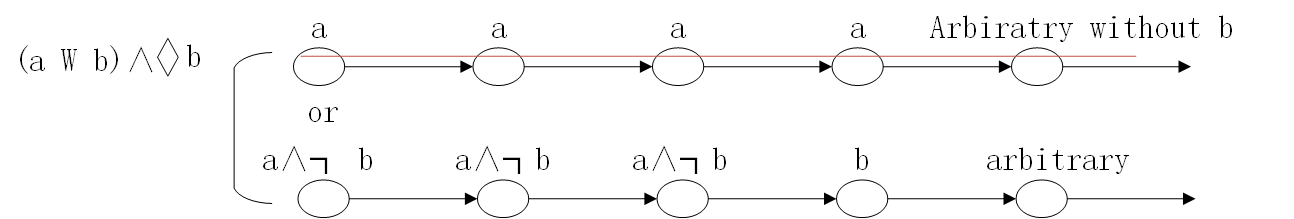
\includegraphics[width=3.0in]{6.png}
      \caption{"(a \textbf{W} b)$\wedge\diamond$b"}
    \end{figure}
    
    Therefore, "(a \textbf{W} b)$\wedge\diamond$b" is equivalent to "a \textbf{U} b", that is $\varphi\textbf{U}\psi\equiv(\varphi\textbf{W}\psi)\wedge\diamond\psi$.
\end{document} 